\chapter{HASIL DAN PEMBAHASAN}

\section{Pengambilan Data Lokasi}

Data yang digunakan adalah data koordinat lokasi yang diekspor melalui Google Earth. Lokasi pada Google Earth ditandai satu per satu dan diekspor ke dalam bentuk spreadsheet. Dapat dilihat pada Lampiran \ref{lampiran1} seluruh nama-nama SMA di Kabupaten Probolinggo beserta koordinat lokasinya. Data tersebut dikumpulkan sebagai dataset dari penelitian ini. Visualisasi data dari koordinat-koordinat SMA di Kabupaten Probolinggo dapat dilihat pada Gambar \ref{fig:petasma}.

\begin{figure}[H]
  \centering
  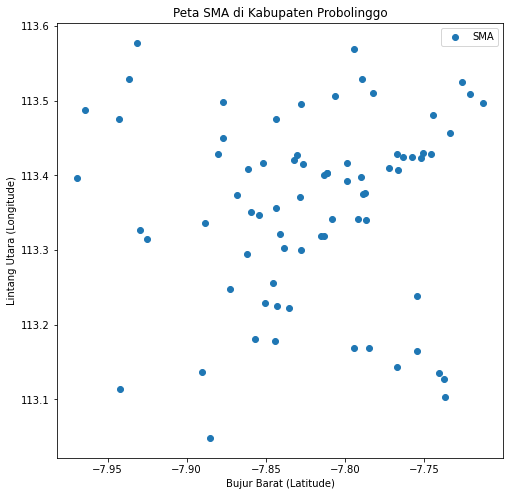
\includegraphics[width=0.5\textwidth]{Gambar/peta sma.png}
  \caption{Visualisasi lokasi SMA di Kabupaten Probolinggo}
  \label{fig:petasma}
\end{figure}

Setelah peneliti mendapatkan lokasi yang akan diproses, selanjutnya diuji menggunakan pembagian dari 1 sampai dengan 10 klaster untuk mengetahui rute dan pembagian klaster yang paling optimal. Berikut ini adalah hasil dari percobaan tersebut.

\section{Proses Pengklasteran Data}

Pada tahap ini metode yang digunakan adalah metode $k$-means untuk mengklaster data dengan tahapan sebagai berikut.

\begin{enumerate}
	\item Tentukan jumlah klaster, dalam hal ini yang digunakan adalah uji coba dengan pembagian 1 sampai dengan 10 klaster.
	\item Selanjutnya pilih titik-titik \textit{centroid} secara acak sebanyak jumlah klaster. Dari hasil pemilihan acak tersebut terpilih titik-titik \textit{centroid} berikut.
	
	\begin{enumerate}
	
	\item Untuk pembagian 1 klaster terpilih titik-titik \textit{centroid} pada Tabel \ref{tab:center1}.
	
\begin{table}[H]
\footnotesize
\centering
\begin{tabular}{ccc}
\rowcolor[HTML]{4472C4} 
{\color[HTML]{FFFFFF} \textbf{Nama Centroid}} & {\color[HTML]{FFFFFF} \textbf{Latitude (Sumbu X)}} & {\color[HTML]{FFFFFF} \textbf{Longitude (Sumbu Y)}} \\
\rowcolor[HTML]{D9E1F2} 
A &
  -7,77 &
  113,41
\end{tabular}
\caption{\textit{Centroid} pada 1 klaster}
\label{tab:center1}
\end{table}

	\item Untuk pembagian 2 klaster terpilih titik-titik \textit{centroid} pada Tabel \ref{tab:center2}.

\begin{table}[H]
\footnotesize
\centering
\begin{tabular}{ccc}
\rowcolor[HTML]{4472C4} 
{\color[HTML]{FFFFFF} \textbf{Nama   Centroid}} & {\color[HTML]{FFFFFF} \textbf{Latitude (Sumbu X)}} & {\color[HTML]{FFFFFF} \textbf{Longitude (Sumbu Y)}} \\
\rowcolor[HTML]{D9E1F2} 
A                                               & -7,75                                              & 113,42                                              \\
B                                               & -7,83                                              & 113,30                                             
\end{tabular}
\caption{\textit{Centroid} pada 2 klaster}
\label{tab:center2}
\end{table}

	\item Untuk pembagian 3 klaster terpilih titik-titik \textit{centroid} pada Tabel \ref{tab:center3}.
	
\begin{table}[H]
\footnotesize
\centering
\begin{tabular}{ccc}
\rowcolor[HTML]{4472C4} 
{\color[HTML]{FFFFFF} \textbf{Nama   Centroid}} & {\color[HTML]{FFFFFF} \textbf{Latitude (Sumbu X)}} & {\color[HTML]{FFFFFF} \textbf{Longitude (Sumbu Y)}} \\
\rowcolor[HTML]{D9E1F2} 
A & -7,84 & 113,22 \\
B & -7,93 & 113,31 \\
\rowcolor[HTML]{D9E1F2} 
C & -7,79 & 113,38
\end{tabular}
\caption{Centroid pada 3 klaster}
\label{tab:center3}
\end{table}

	\item Untuk pembagian 4 klaster terpilih titik-titik \textit{centroid} pada Tabel \ref{tab:center4}.
	
\begin{table}[H]
\footnotesize
\centering
\begin{tabular}{ccc}
\rowcolor[HTML]{4472C4} 
{\color[HTML]{FFFFFF} \textbf{Nama   Centroid}} & {\color[HTML]{FFFFFF} \textbf{Latitude (Sumbu X)}} & {\color[HTML]{FFFFFF} \textbf{Longitude (Sumbu Y)}} \\
\rowcolor[HTML]{D9E1F2} 
A & -7,77 & 113,43 \\
B & -7,83 & 113,42 \\
\rowcolor[HTML]{D9E1F2} 
C & -7,74 & 113,13 \\
D & -7,75 & 113,42
\end{tabular}
\caption{\textit{Centroid} pada 4 klaster}
\label{tab:center4}
\end{table}	
	
	\item Untuk pembagian 5 klaster terpilih titik-titik \textit{centroid} pada Tabel \ref{tab:center5}
	
\begin{table}[H]
\footnotesize
\centering
\begin{tabular}{ccc}
\rowcolor[HTML]{4472C4} 
{\color[HTML]{FFFFFF} \textbf{Nama   Centroid}} & {\color[HTML]{FFFFFF} \textbf{Latitude (Sumbu X)}} & {\color[HTML]{FFFFFF} \textbf{Longitude (Sumbu Y)}} \\
\rowcolor[HTML]{D9E1F2} 
A & -7,94 & 113,11 \\
B & -7,85 & 113,42 \\
\rowcolor[HTML]{D9E1F2} 
C & -7,80 & 113,39 \\
D & -7,94 & 113,53 \\
\rowcolor[HTML]{D9E1F2} 
E & -7,84 & 113,32
\end{tabular}
\caption{\textit{Centroid} pada 5 klaster}
\label{tab:center5}
\end{table}

	\item Untuk pembagian 6 klaster terpilih titik-titik \textit{centroid} pada Tabel \ref{tab:center6}.
	
\begin{table}[H]
\footnotesize
\centering
\begin{tabular}{ccc}
\rowcolor[HTML]{4472C4} 
{\color[HTML]{FFFFFF} \textbf{Nama   Centroid}} & {\color[HTML]{FFFFFF} \textbf{Latitude (Sumbu X)}} & {\color[HTML]{FFFFFF} \textbf{Longitude (Sumbu Y)}} \\
\rowcolor[HTML]{D9E1F2} 
A & -7,79 & 113,53 \\
B & -7,86 & 113,29 \\
\rowcolor[HTML]{D9E1F2} 
C & -7,89 & 113,14 \\
D & -7,87 & 113,37 \\
\rowcolor[HTML]{D9E1F2} 
E & -7,94 & 113,48 \\
F & -7,88 & 113,50
\end{tabular}
\caption{\textit{Centroid} pada 6 klaster}
\label{tab:center6}
\end{table}

	\item Untuk pembagian 7 klaster terpilih titik-titik \textit{centroid} pada Tabel \ref{tab:center7}.
	
\begin{table}[H]
\footnotesize
\centering
\begin{tabular}{ccc}
\rowcolor[HTML]{4472C4} 
{\color[HTML]{FFFFFF} \textbf{Nama   Centroid}} & {\color[HTML]{FFFFFF} \textbf{Latitude (Sumbu X)}} & {\color[HTML]{FFFFFF} \textbf{Longitude (Sumbu Y)}} \\
\rowcolor[HTML]{D9E1F2} 
A & -7,89 & 113,34 \\
B & -7,81 & 113,32 \\
\rowcolor[HTML]{D9E1F2} 
C & -7,84 & 113,48 \\
D & -7,79 & 113,17 \\
\rowcolor[HTML]{D9E1F2} 
E & -7,71 & 113,50 \\
F & -7,77 & 113,41 \\
\rowcolor[HTML]{D9E1F2} 
G & -7,72 & 113,51
\end{tabular}
\caption{\textit{Centroid} pada 7 klaster}
\label{tab:center7}
\end{table}

	\item Untuk pembagian 8 klaster terpilih titik-titik \textit{centroid} pada Tabel \ref{tab:center8}.

\begin{table}[H]
\footnotesize
\centering
\begin{tabular}{ccc}
\rowcolor[HTML]{4472C4} 
{\color[HTML]{FFFFFF} \textbf{Nama   Centroid}} & {\color[HTML]{FFFFFF} \textbf{Latitude (Sumbu X)}} & {\color[HTML]{FFFFFF} \textbf{Longitude (Sumbu Y)}} \\
\rowcolor[HTML]{D9E1F2} 
A & -7,79 & 113,38 \\
B & -7,88 & 113,43 \\
\rowcolor[HTML]{D9E1F2} 
C & -7,78 & 113,51 \\
D & -7,84 & 113,30 \\
\rowcolor[HTML]{D9E1F2} 
E & -7,75 & 113,43 \\
F & -7,75 & 113,16 \\
\rowcolor[HTML]{D9E1F2} 
G & -7,86 & 113,18 \\
H & -7,86 & 113,35
\end{tabular}
\caption{\textit{Centroid} pada 8 klaster}
\label{tab:center8}
\end{table}

	\item Untuk pembagian 9 klaster terpilih titik-titik \textit{centroid} pada Tabel \ref{tab:center9}.
	
\begin{table}[H]
\footnotesize
\centering
\begin{tabular}{ccc}
\rowcolor[HTML]{4472C4} 
{\color[HTML]{FFFFFF} \textbf{Nama   Centroid}} & {\color[HTML]{FFFFFF} \textbf{Latitude (Sumbu X)}} & {\color[HTML]{FFFFFF} \textbf{Longitude (Sumbu Y)}} \\
\rowcolor[HTML]{D9E1F2} 
A & -7,83 & 113,30 \\
B & -7,74 & 113,48 \\
\rowcolor[HTML]{D9E1F2} 
C & -7,84 & 113,22 \\
D & -7,93 & 113,31 \\
\rowcolor[HTML]{D9E1F2} 
E & -7,79 & 113,38 \\
F & -7,88 & 113,43 \\
\rowcolor[HTML]{D9E1F2} 
G & -7,78 & 113,51 \\
H & -7,84 & 113,30 \\
\rowcolor[HTML]{D9E1F2} 
I & -7,75 & 113,43 \\                        
\end{tabular}
\caption{\textit{Centroid} pada 9 klaster}
\label{tab:center9}
\end{table}

	\item Untuk pembagian 10 klaster terpilih titik-titik \textit{centroid} pada Tabel \ref{tab:center10}.
	
\begin{table}[H]
\centering
\footnotesize
\begin{tabular}{ccc}
\rowcolor[HTML]{4472C4} 
{\color[HTML]{FFFFFF} \textbf{Nama   Centroid}} & {\color[HTML]{FFFFFF} \textbf{Latitude (Sumbu X)}} & {\color[HTML]{FFFFFF} \textbf{Longitude (Sumbu Y)}} \\
\rowcolor[HTML]{D9E1F2} 
A & -7,77 & 113,41 \\
B & -7,76 & 113,43 \\
\rowcolor[HTML]{D9E1F2} 
C & -7,84 & 113,18 \\
D & -7,83 & 113,50 \\
\rowcolor[HTML]{D9E1F2} 
E & -7,87 & 113,25 \\
F & -7,94 & 113,11 \\
\rowcolor[HTML]{D9E1F2} 
G & -7,85 & 113,42 \\
H & -7,80 & 113,39 \\
\rowcolor[HTML]{D9E1F2} 
I & -7,94 & 113,53 \\
J & -7,84 & 113,32
\end{tabular}
\caption{Centroid pada 10 klaster}
\label{tab:center10}
\end{table}

		
	\end{enumerate}

	\item \label{ulang3} Hitung jarak tiap titik sekolah yang ada dengan masing-masing titik \textit{centroid}. Penghitungan jarak menggunakan \textit{Euclidean distance} pada persamaan (\ref{eq:euclidean}).
	
	\item Kelompokan data ke dalam klaster yang memiliki jarak paling minimum.
	\item Setelah seluruh titik sekolah masuk ke dalam klaster-klaster, hitung \textit{centroid} yang baru dengan cara menghitung rata-rata titik sekolah yang ada di dalam klaster tersebut. Lakukan hal yang sama pada klaster yang lain.
	\item Jika terdapat perubahan klaster, maka ulang langkah \ref{ulang3} hingga tidak ada perubahan anggota pada tiap klaster. Jika \textit{centroid} yang baru tidak berubah dari sebelumnya, maka proses berhenti, karena \textit{centroid} yang tidak berubah menyebabkan anggota klaster juga tidak berubah.
	
	\item Setelah semua data terklaster, selanjutnya adalah menentukan titik asal dengan cara menghitung rata-rata dari seluruh titik-titik \textit{centroid} tersebut.
\end{enumerate}

Dari serangkaian proses $k$-means menghasilkan klaster-klaster berbeda. Data-data tersebut telah berhasil dikelompokkan, selanjutnya data tersebut akan diproses untuk ke tahapan selanjutnya.

\section{Proses TSP Menggunakan Algoritma Genetika}

Setelah data terklaster seperti pada Gambar \ref{fig:hasilklas} selanjutnya adalah mencari rute terdekatnya menggunakan algoritma genetika.

\begin{figure}[H]
	\centering
	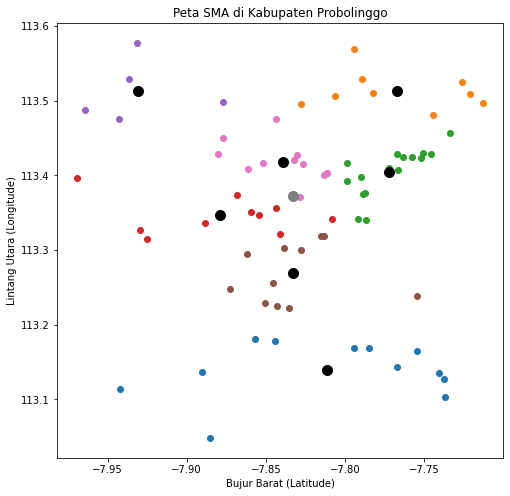
\includegraphics[width=0.5\textwidth]{Gambar/hasil klaster.png}
	\caption{Visualisasi klaster sesuai warna}
	\label{fig:hasilklas}
\end{figure}

\begin{enumerate}
	\item Pada tahap awal, populasi yang berisi sejumlah kromosom yang di dalamnya dibangkitkan.
	\item \label{ulang4} Selanjutnya adalah menghitung nilai \textit{fitness} dari populasi yang dihasilkan, yaitu menghitung nilai total jarak dari masing-masing kromosom.
	\item Setelah nilai \textit{fitness} ditemukan, selanjutnya menetapkan probabilitas \textit{crossover} ($p_c$), dalam hal ini yang digunakan adalah $p_c=0,95$. Bangkitkan bilangan acak (0,0000 sampai 1,0000) pada setiap kromosom, kromosom dengan bilangan acak kurang dari $p_c$ maka akan dilakukan \textit{crossover}. Jika kromosom hasil \textit{crossover} memiliki \textit{fitness} yang lebih baik  dari kromosom awal, maka kromosom awal digantikan oleh kromosom hasil \textit{crossover}.
	\item Langkah selanjutnya adalah menentukan probabilitas mutasi ($p_m$), dalam menentukan probabilitah mutasi yang digunakan adalah $p_m=0,1$. Bangkitkan bilangan acak (0,0000 sampai 1,0000) pada setiap kromosom, kromosom yang memiliki bilangan acak kurang dari $p_m$ maka akan dilakukan mutasi. Jika kromosom hasil mutasi memiliki \textit{fitness} yang lebih baik dari kromosom awal, maka kromosom awal digantikan oleh kromosom hasil mutasi.
	\item Iterasi dilakukan dengan cara kembali ke tahapan \ref{ulang4} untuk generasi berikutnya sampai hasil yang dilakukan optimal atau mendekati optimal.
\end{enumerate}

\section{Hasil Dari Proses MTSP}

Dari serangkaian proses di atas, menghasilkan beberapa rute optimal yang dapat dilalui yang merupakan rute yang didapatkan dari pembagian klaster berbeda. Salah satunya pada Gambar \ref{fig:hasil_mtsp1} tidak menggunakan pembagian klaster, sehingga titik \textit{centroid} pada klaster tersebut dijadikan titik asal.

Rute-rute yang dihasilkan sebelumnya diekspor ke bentuk spreadsheet dan telah diurutkan berdasarkan nomor urut yang terdapat pada Lampiran \ref{lampiran1} sehingga mempermudah pengguna dalam membaca data.

\subsection{Tanpa pembagian klaster}

Urutan perjalanan perjalanan dengan tanpa pembagian klaster menghasilkan urutan titik seperti berikut. $K$-means pada urutan ini tidak digunakan untuk pengklasteran data, namun hanya untuk penentuan titik asal.

$67\rightarrow65\rightarrow53\rightarrow27\rightarrow4\rightarrow42\rightarrow66\rightarrow34\rightarrow70\rightarrow8\rightarrow19\rightarrow28\rightarrow37\rightarrow11\rightarrow25\rightarrow72\rightarrow55\rightarrow31\rightarrow3\rightarrow74\rightarrow15\rightarrow68\rightarrow20\rightarrow44\rightarrow40\rightarrow16\rightarrow30\rightarrow23\rightarrow24\rightarrow63\rightarrow13\rightarrow29\rightarrow50\rightarrow7\rightarrow54\rightarrow2\rightarrow10\rightarrow52\rightarrow64\rightarrow21\rightarrow62\rightarrow58\rightarrow26\rightarrow1\rightarrow69\rightarrow14\rightarrow45\rightarrow61\rightarrow38\rightarrow59\rightarrow17\rightarrow71\rightarrow18\rightarrow32\rightarrow57\rightarrow73\rightarrow75\rightarrow41\rightarrow39\rightarrow49\rightarrow51\rightarrow6\rightarrow60\rightarrow22\rightarrow33\rightarrow48\rightarrow5\rightarrow35\rightarrow46\rightarrow56\rightarrow36\rightarrow47\rightarrow9\rightarrow12\rightarrow43$

Urutan perjalanan menuju seluruh SMA di Kabupaten Probolinggo tanpa pembagian klaster, dapat dilihat pada Gambar \ref{fig:hasil_mtsp1}. Urutan tersebut tampaknya masih belum sepenuhnya optimal, karena menghasilkan jarak total yang dilalui oleh \textit{salesman} yaitu $10,05030304$ satuan dengan koordinat titik asal yaitu $(7.82, 113.35)$ dapat dilihat pada Tabel \ref{tab:totaljarak}.

\begin{figure}[H]
\centering
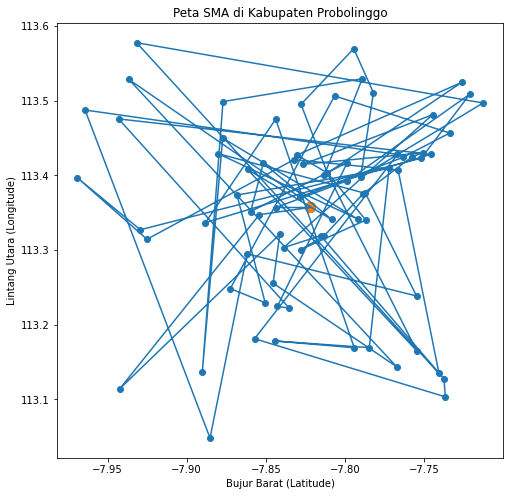
\includegraphics[width=0.5\textwidth]{Gambar/hasil_mtsp/1}
\caption{Perjalanan tanpa pembagian klaster}
\label{fig:hasil_mtsp1}
\end{figure}

\subsection{Pembagian 2 klaster}

Pada tahap ini urutan perjalanan dibagi menjadi 2 klaster yaitu klaster A dan B, menghasilkan urutan sebagai berikut.

\begin{enumerate}
\item Urutan perjalanan pada klaster A:

$33\rightarrow52\rightarrow21\rightarrow32\rightarrow55\rightarrow36\rightarrow10\rightarrow37\rightarrow56\rightarrow30\rightarrow27\rightarrow59\rightarrow60\rightarrow64\rightarrow6\rightarrow39\rightarrow24\rightarrow72\rightarrow13\rightarrow29\rightarrow11\rightarrow63\rightarrow9\rightarrow17\rightarrow47\rightarrow38$

\item Urutan perjalanan pada klaster B:

$57\rightarrow58\rightarrow71\rightarrow53\rightarrow49\rightarrow25\rightarrow16\rightarrow23\rightarrow46\rightarrow35\rightarrow61\rightarrow15\rightarrow4\rightarrow41\rightarrow44\rightarrow48\rightarrow67\rightarrow45\rightarrow69\rightarrow5\rightarrow8\rightarrow42\rightarrow50\rightarrow22\rightarrow51\rightarrow74\rightarrow26\rightarrow19\rightarrow34\rightarrow43\rightarrow65\rightarrow12\rightarrow28\rightarrow14\rightarrow70\rightarrow66\rightarrow3\rightarrow40\rightarrow20\rightarrow62\rightarrow31\rightarrow18\rightarrow7\rightarrow54\rightarrow68\rightarrow73\rightarrow75\rightarrow2\rightarrow1$

\end{enumerate}

Urutan perjalanan menuju seluruh SMA di Kabupaten Probolinggo dengan dibagi menjadi 2 klaster, dapat dilihat pada Gambar \ref{fig:hasil_mtsp2}. Urutan tersebut menghasilkan jarak total yang dilalui oleh \textit{salesman} yaitu $6,858777424$ satuan dengan koordinat titik asal yaitu $(7.82, 113.32)$ dapat dilihat pada Tabel \ref{tab:totaljarak}.


\begin{figure}[H]
\centering
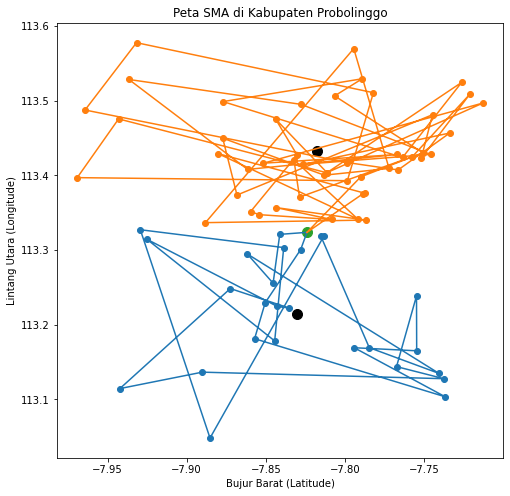
\includegraphics[width=0.5\textwidth]{Gambar/hasil_mtsp/2}
\caption{Perjalanan dibagi 2 klaster}
\label{fig:hasil_mtsp2}
\end{figure}

\subsection{Pembagian 3 klaster}

Pada tahap ini urutan perjalanan dibagi menjadi 3 klaster yaitu klaster A, B, dan C, menghasilkan urutan perjalanan sebagai berikut.

\begin{enumerate}
\item Urutan perjalanan pada klaster A:

$38\rightarrow60\rightarrow56\rightarrow32\rightarrow13\rightarrow47\rightarrow37\rightarrow29\rightarrow55\rightarrow59\rightarrow17\rightarrow30\rightarrow11\rightarrow27\rightarrow21\rightarrow72\rightarrow36\rightarrow10$

\item Urutan perjalanan pada klaster B:

$50\rightarrow41\rightarrow44\rightarrow42\rightarrow34\rightarrow2\rightarrow66\rightarrow14\rightarrow8\rightarrow70\rightarrow28\rightarrow51\rightarrow26\rightarrow74\rightarrow54\rightarrow22\rightarrow7$

\item Urutan perjalanan pada klaster C:

$65\rightarrow48\rightarrow35\rightarrow1\rightarrow46\rightarrow40\rightarrow4\rightarrow45\rightarrow43\rightarrow18\rightarrow49\rightarrow53\rightarrow62\rightarrow5\rightarrow71\rightarrow73\rightarrow19\rightarrow61\rightarrow57\rightarrow63\rightarrow15\rightarrow25\rightarrow68\rightarrow58\rightarrow24\rightarrow31\rightarrow16\rightarrow3\rightarrow12\rightarrow20\rightarrow52\rightarrow67\rightarrow69\rightarrow75\rightarrow39\rightarrow6\rightarrow64\rightarrow23\rightarrow33\rightarrow9$

\end{enumerate}

Urutan perjalanan menuju seluruh SMA di Kabupaten Probolinggo dengan dibagi menjadi 3 klaster, dapat dilihat pada Gambar \ref{fig:hasil_mtsp3}. Pada urutan tersebut menghasilkan jarak total yang dilalui oleh \textit{salesman} yaitu $5,599877636$ satuan dengan koordinat titik asal yaitu $(7.82, 113.35)$ dapat dilihat pada Tabel \ref{tab:totaljarak}.

\begin{figure}[H]
\centering
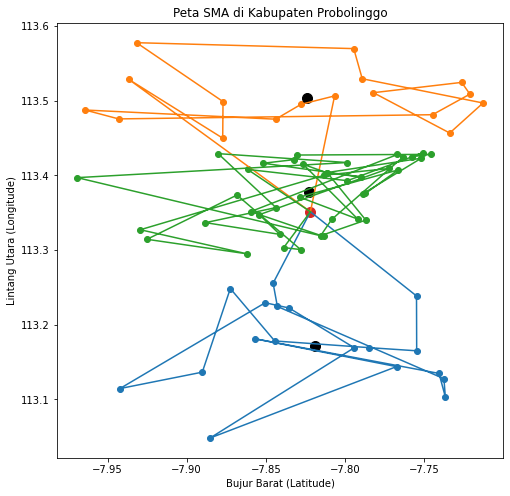
\includegraphics[width=0.5\textwidth]{Gambar/hasil_mtsp/3}
\caption{Perjalanan dibagi 3 klaster}
\label{fig:hasil_mtsp3}
\end{figure}

\subsection{Pembagian 4 klaster}

Pada tahap ini urutan perjalanan dibagi menjadi 4 klaster yaitu klaster A, B, C, dan D, menghasilkan urutan perjalanan sebagai berikut.

\begin{enumerate}

\item Urutan perjalanan pada klaster A:

$60\rightarrow36\rightarrow55\rightarrow32\rightarrow56\rightarrow37\rightarrow29\rightarrow13\rightarrow27\rightarrow38\rightarrow59\rightarrow17\rightarrow72\rightarrow21\rightarrow30\rightarrow11\rightarrow47\rightarrow10$

\item Urutan perjalanan pada klaster B:

$22\rightarrow44\rightarrow50\rightarrow42\rightarrow54\rightarrow2\rightarrow51\rightarrow66\rightarrow70\rightarrow28\rightarrow34\rightarrow8\rightarrow7$

\item Urutan perjalanan pada klaster C:

$48\rightarrow68\rightarrow1\rightarrow14\rightarrow19\rightarrow69\rightarrow5\rightarrow18\rightarrow61\rightarrow73\rightarrow71\rightarrow16\rightarrow46\rightarrow35\rightarrow25\rightarrow53\rightarrow15\rightarrow43\rightarrow75\rightarrow4\rightarrow49\rightarrow40\rightarrow57$

\item Urutan perjalanan pada klaster D:

$23\rightarrow62\rightarrow58\rightarrow31\rightarrow63\rightarrow9\rightarrow6\rightarrow65\rightarrow45\rightarrow33\rightarrow64\rightarrow39\rightarrow41\rightarrow74\rightarrow26\rightarrow20\rightarrow24\rightarrow67\rightarrow12\rightarrow3\rightarrow52$

\end{enumerate}

Urutan perjalanan menuju seluruh SMA di Kabupaten Probolinggo dengan dibagi menjadi 4 klaster, dapat dilihat pada Gambar \ref{fig:hasil_mtsp4}. Pada urutan tersebut menghasilkan jarak total yang dilalui oleh \textit{salesman} yaitu $5,010993898$ satuan dengan koordinat titik asal yaitu $(7.82, 113.36)$ dapat dilihat pada Tabel \ref{tab:totaljarak}.


\begin{figure}[H]
\centering
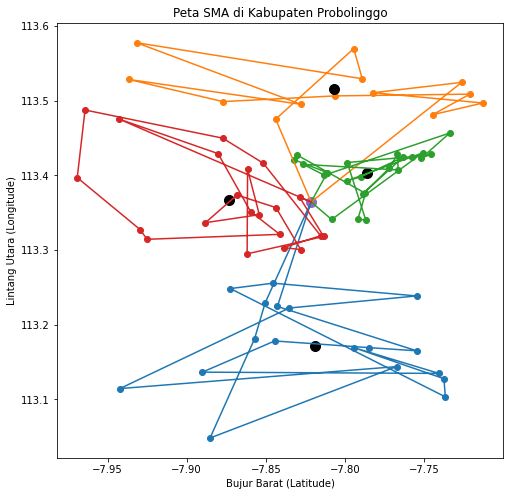
\includegraphics[width=0.5\textwidth]{Gambar/hasil_mtsp/4}
\caption{Perjalanan dibagi 4 klaster}
\label{fig:hasil_mtsp4}
\end{figure}

\subsection{Pembagian 5 klaster}

Pada tahap ini urutan perjalanan dibagi menjadi 5 klaster yaitu klaster A, B, C, D, dan E, menghasilkan urutan perjalanan sebagai berikut.

\begin{enumerate}

\item Urutan perjalanan pada klaster A:

$37\rightarrow36\rightarrow13\rightarrow55\rightarrow21\rightarrow30\rightarrow29\rightarrow72\rightarrow47\rightarrow56\rightarrow32\rightarrow10\rightarrow11\rightarrow17\rightarrow59\rightarrow60$

\item Urutan perjalanan pada klaster B:

$22\rightarrow7\rightarrow28\rightarrow70\rightarrow8\rightarrow34\rightarrow2\rightarrow66\rightarrow51\rightarrow14$

\item Urutan perjalanan pada klaster C:

$49\rightarrow75\rightarrow19\rightarrow1\rightarrow35\rightarrow46\rightarrow61\rightarrow69\rightarrow73\rightarrow71\rightarrow43\rightarrow40\rightarrow48\rightarrow53\rightarrow57\rightarrow25\rightarrow45\rightarrow65\rightarrow5\rightarrow18\rightarrow68\rightarrow16\rightarrow4\rightarrow62$

\item Urutan perjalanan pada klaster D:

$15\rightarrow27\rightarrow6\rightarrow52\rightarrow24\rightarrow64\rightarrow39\rightarrow20\rightarrow9\rightarrow38\rightarrow33\rightarrow63\rightarrow12\rightarrow23\rightarrow67\rightarrow58$

\item Urutan perjalanan pada klaster E:

$74\rightarrow26\rightarrow50\rightarrow42\rightarrow54\rightarrow44\rightarrow3\rightarrow41\rightarrow31$

\end{enumerate}

Urutan perjalanan menuju seluruh SMA di Kabupaten Probolinggo dengan dibagi menjadi 5 klaster, dapat dilihat pada Gambar \ref{fig:hasil_mtsp5}. Pada urutan tersebut menghasilkan jarak total yang dilalui oleh \textit{salesman} yaitu $4,805014746$ satuan dengan koordinat titik asal yaitu $(7.82, 113.37)$ dapat dilihat pada Tabel \ref{tab:totaljarak}.

\begin{figure}[H]
\centering
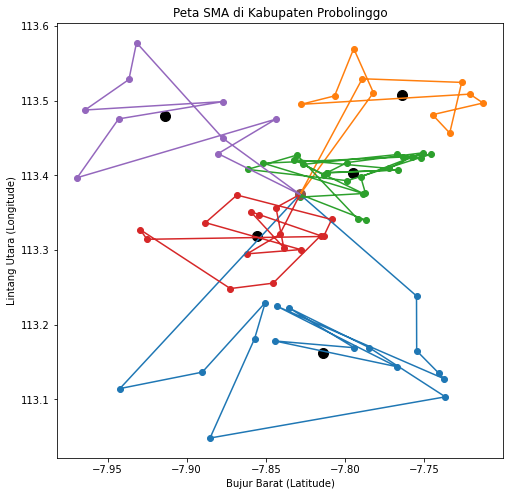
\includegraphics[width=0.5\textwidth]{Gambar/hasil_mtsp/5}
\caption{Perjalanan dibagi 5 klaster}
\label{fig:hasil_mtsp5}
\end{figure}

\subsection{Pembagian 6 klaster}

Pada tahap ini urutan perjalanan dibagi menjadi 6 klaster yaitu klaster A, B, C, D, E, dan F, menghasilkan urutan perjalanan sebagai berikut.

\begin{enumerate}

\item Urutan perjalanan pada klaster A:

$13\rightarrow29\rightarrow30\rightarrow11\rightarrow32\rightarrow56\rightarrow36\rightarrow37\rightarrow72\rightarrow55$

\item Urutan perjalanan pada klaster B:

$14\rightarrow70\rightarrow28\rightarrow66\rightarrow51\rightarrow2\rightarrow34\rightarrow8\rightarrow22\rightarrow7$

\item Urutan perjalanan pada klaster C:

$4\rightarrow40\rightarrow69\rightarrow16\rightarrow49\rightarrow68\rightarrow25\rightarrow19\rightarrow46\rightarrow35\rightarrow43\rightarrow71\rightarrow48\rightarrow75\rightarrow18\rightarrow61\rightarrow73\rightarrow5\rightarrow1\rightarrow45\rightarrow65$

\item Urutan perjalanan pada klaster D:

$62\rightarrow9\rightarrow67\rightarrow57\rightarrow53\rightarrow15\rightarrow23\rightarrow58\rightarrow20\rightarrow39\rightarrow64\rightarrow52\rightarrow12\rightarrow6\rightarrow24\rightarrow63\rightarrow33$

\item Urutan perjalanan pada klaster E:

$44\rightarrow54\rightarrow74\rightarrow42\rightarrow50\rightarrow26\rightarrow31\rightarrow3\rightarrow41$

\item Urutan perjalanan pada klaster F:

$17\rightarrow60\rightarrow59\rightarrow38\rightarrow27\rightarrow47\rightarrow21\rightarrow10$

\end{enumerate}

Urutan perjalanan menuju seluruh SMA di Kabupaten Probolinggo dengan dibagi menjadi 6 klaster, dapat dilihat pada Gambar \ref{fig:hasil_mtsp6}. Pada urutan tersebut menghasilkan jarak total yang dilalui oleh \textit{salesman} yaitu $4,431319949$ satuan dengan koordinat titik asal yaitu $(7.82, 113.34)$ dapat dilihat pada Tabel \ref{tab:totaljarak}.

\begin{figure}[H]
\centering
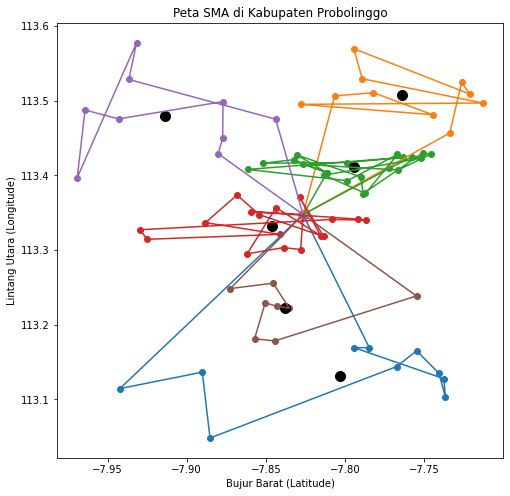
\includegraphics[width=0.5\textwidth]{Gambar/hasil_mtsp/6}
\caption{Perjalanan dibagi 6 klaster}
\label{fig:hasil_mtsp6}
\end{figure}

\subsection{Pembagian 7 klaster}

Pada tahap ini urutan perjalanan dibagi menjadi 7 klaster yaitu klaster A, B, C, D, E, F, dan G, menghasilkan urutan perjalanan sebagai berikut.

\begin{enumerate}

\item Urutan perjalanan pada klaster A:

$11\rightarrow30\rightarrow29\rightarrow47\rightarrow21\rightarrow72\rightarrow32\rightarrow56\rightarrow13\rightarrow37\rightarrow55\rightarrow36$

\item Urutan perjalanan pada klaster B:

$7\rightarrow70\rightarrow66\rightarrow28\rightarrow51\rightarrow8\rightarrow2\rightarrow34\rightarrow22$

\item Urutan perjalanan pada klaster C:

$1\rightarrow19\rightarrow73\rightarrow48\rightarrow69\rightarrow35\rightarrow46\rightarrow68\rightarrow25\rightarrow16\rightarrow5\rightarrow14\rightarrow43\rightarrow71\rightarrow53\rightarrow57$

\item Urutan perjalanan pada klaster D:

$67\rightarrow58\rightarrow23\rightarrow12\rightarrow20\rightarrow64\rightarrow39\rightarrow31\rightarrow52\rightarrow15$

\item Urutan perjalanan pada klaster E:

$26\rightarrow44\rightarrow50\rightarrow42\rightarrow74$

\item Urutan perjalanan pada klaster F:

$24\rightarrow63\rightarrow10\rightarrow59\rightarrow60\rightarrow17\rightarrow33\rightarrow9\rightarrow38\rightarrow27\rightarrow6$

\item Urutan perjalanan pada klaster G:

$40\rightarrow49\rightarrow54\rightarrow4\rightarrow41\rightarrow3\rightarrow45\rightarrow61\rightarrow18\rightarrow75\rightarrow65\rightarrow62$

\end{enumerate}

Urutan perjalanan menuju seluruh SMA di Kabupaten Probolinggo dengan dibagi menjadi 7 klaster, dapat dilihat pada Gambar \ref{fig:hasil_mtsp7}. Pada urutan tersebut menghasilkan jarak total yang dilalui oleh \textit{salesman} yaitu $4,353294633$ satuan dengan koordinat titik asal yaitu $(7.82, 113.37)$ dapat dilihat pada Tabel \ref{tab:totaljarak}. Nilai jarak total pada pembagian klaster ini merupakan jarak total yang paling rendah diantara yang lain.

\begin{figure}[H]
\centering
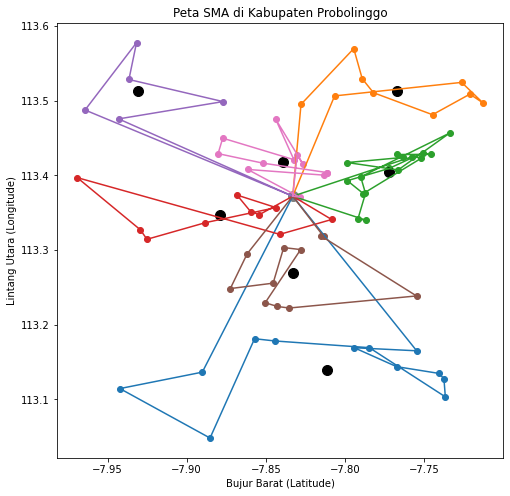
\includegraphics[width=0.5\textwidth]{Gambar/hasil_mtsp/7}
\caption{Perjalanan dibagi 7 klaster}
\label{fig:hasil_mtsp7}
\end{figure}

\subsection{Pembagian 8 klaster}

Pada tahap ini urutan perjalanan dibagi menjadi 8 klaster yaitu klaster A, B, C, D, E, F, G, dan H, menghasilkan urutan perjalanan sebagai berikut.

\begin{enumerate}
\item Urutan perjalanan pada klaster A:

$11\rightarrow47\rightarrow21\rightarrow37\rightarrow13\rightarrow32\rightarrow56\rightarrow36\rightarrow72\rightarrow55\rightarrow29\rightarrow30$

\item Urutan perjalanan pada klaster B:

$22\rightarrow7\rightarrow51\rightarrow66\rightarrow28\rightarrow2\rightarrow34\rightarrow70\rightarrow8$

\item Urutan perjalanan pada klaster C:

$43\rightarrow5\rightarrow19\rightarrow35\rightarrow25\rightarrow69\rightarrow68\rightarrow46\rightarrow14\rightarrow16\rightarrow1\rightarrow48$

\item Urutan perjalanan pada klaster D:

$39\rightarrow64\rightarrow20\rightarrow31\rightarrow23$

\item Urutan perjalanan pada klaster E:

$26\rightarrow74\rightarrow50\rightarrow42\rightarrow44$

\item Urutan perjalanan pada klaster F:

$33\rightarrow10\rightarrow59\rightarrow17\rightarrow60\rightarrow27\rightarrow38\rightarrow6\rightarrow9$

\item Urutan perjalanan pada klaster G:

$61\rightarrow18\rightarrow75\rightarrow49\rightarrow65\rightarrow3\rightarrow54\rightarrow41\rightarrow45\rightarrow40\rightarrow4$

\item Urutan perjalanan pada klaster H:

$53\rightarrow67\rightarrow52\rightarrow12\rightarrow24\rightarrow57\rightarrow58\rightarrow63\rightarrow15\rightarrow73\rightarrow71\rightarrow62$
\end{enumerate}

Urutan perjalanan menuju seluruh SMA di Kabupaten Probolinggo dengan dibagi menjadi 8 klaster, dapat dilihat pada Gambar \ref{fig:hasil_mtsp8}. Pada urutan tersebut menghasilkan jarak total yang dilalui oleh \textit{salesman} yaitu $4,398984127$ satuan dengan koordinat titik asal yaitu $(7.83, 113.35)$ dapat dilihat pada Tabel \ref{tab:totaljarak}.

\begin{figure}[H]
\centering
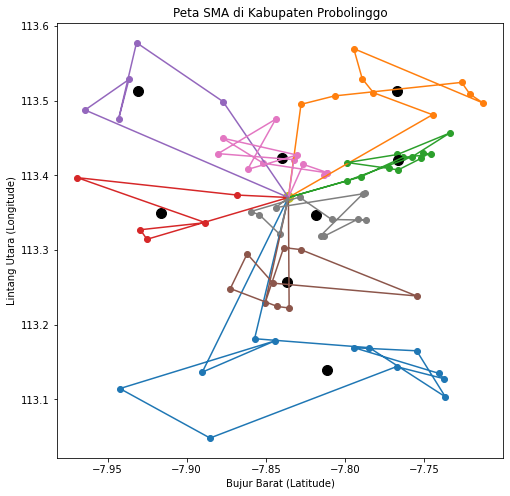
\includegraphics[width=0.5\textwidth]{Gambar/hasil_mtsp/8}
\caption{Perjalanan dibagi 8 klaster}
\label{fig:hasil_mtsp8}
\end{figure}

\subsection{Pembagian 9 klaster}

Pada tahap ini urutan perjalanan dibagi menjadi 9 klaster yaitu klaster A, B, C, D, E, F, G, H, dan I, menghasilkan urutan perjalanan sebagai berikut.

\begin{enumerate}
\item Urutan perjalanan pada klaster A:

$17\rightarrow60\rightarrow21\rightarrow47\rightarrow59\rightarrow10$

\item Urutan perjalanan pada klaster B:

$28\rightarrow66\rightarrow70\rightarrow8\rightarrow51\rightarrow34\rightarrow2\rightarrow7\rightarrow22$

\item Urutan perjalanan pada klaster C:

$16\rightarrow5\rightarrow25\rightarrow69\rightarrow35\rightarrow46\rightarrow14\rightarrow19\rightarrow68\rightarrow1\rightarrow43$

\item Urutan perjalanan pada klaster D:

$39\rightarrow67\rightarrow64\rightarrow20\rightarrow58\rightarrow23\rightarrow31$

\item Urutan perjalanan pada klaster E:

$74\rightarrow26\rightarrow50\rightarrow42\rightarrow44$

\item Urutan perjalanan pada klaster F:

$52\rightarrow9\rightarrow27\rightarrow38\rightarrow6\rightarrow33$

\item Urutan perjalanan pada klaster G:

$75\rightarrow61\rightarrow18\rightarrow3\rightarrow54\rightarrow41\rightarrow40\rightarrow4\rightarrow49\rightarrow45\rightarrow65$

\item Urutan perjalanan pada klaster H:

$48\rightarrow73\rightarrow71\rightarrow62\rightarrow12\rightarrow57\rightarrow24\rightarrow63\rightarrow53\rightarrow15$

\item Urutan perjalanan pada klaster I:

$37\rightarrow56\rightarrow32\rightarrow13\rightarrow11\rightarrow30\rightarrow29\rightarrow36\rightarrow72\rightarrow55$

\end{enumerate}

Urutan perjalanan menuju seluruh SMA di Kabupaten Probolinggo dengan dibagi menjadi 9 klaster, dapat dilihat pada Gambar \ref{fig:hasil_mtsp9}. Pada urutan tersebut menghasilkan jarak total yang dilalui oleh \textit{salesman} yaitu $4,482429562$ satuan dengan koordinat titik asal yaitu $(7.83, 113.35)$ dapat dilihat pada Tabel \ref{tab:totaljarak}.

\begin{figure}[H]
\centering
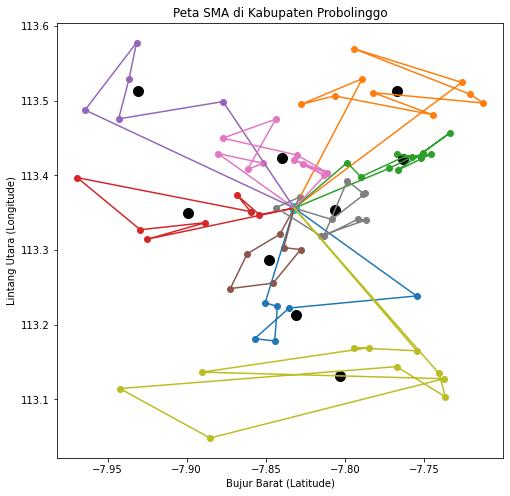
\includegraphics[width=0.5\textwidth]{Gambar/hasil_mtsp/9}
\caption{Perjalanan dibagi 9 klaster}
\label{fig:hasil_mtsp9}
\end{figure}

\subsection{Pembagian 10 klaster}

Pada tahap ini urutan perjalanan dibagi menjadi 10 klaster yaitu klaster A, B, C, D, E, F, G, H, I, dan J, menghasilkan urutan perjalanan sebagai berikut.

\begin{enumerate}
\item Urutan perjalanan pada klaster A:

$10\rightarrow21\rightarrow47\rightarrow17\rightarrow60\rightarrow59$

\item Urutan perjalanan pada klaster B:

$28\rightarrow66\rightarrow70\rightarrow22\rightarrow51\rightarrow2\rightarrow34\rightarrow8\rightarrow7$

\item Urutan perjalanan pada klaster C:

$5\rightarrow68\rightarrow25\rightarrow1\rightarrow35\rightarrow46\rightarrow14\rightarrow19\rightarrow69\rightarrow43\rightarrow16$

\item Urutan perjalanan pada klaster D:

$67\rightarrow20\rightarrow58\rightarrow23\rightarrow39\rightarrow64\rightarrow12\rightarrow52$

\item Urutan perjalanan pada klaster E:

$31\rightarrow74\rightarrow26$

\item Urutan perjalanan pada klaster F:

$38\rightarrow27\rightarrow6\rightarrow9\rightarrow33$

\item Urutan perjalanan pada klaster G:

$18\rightarrow75\rightarrow54\rightarrow41\rightarrow3\rightarrow45\rightarrow65\rightarrow4\rightarrow40\rightarrow49\rightarrow61$

\item Urutan perjalanan pada klaster H:

$62\rightarrow73\rightarrow71\rightarrow48\rightarrow53\rightarrow57\rightarrow15\rightarrow63\rightarrow24$

\item Urutan perjalanan pada klaster I:

$30\rightarrow11\rightarrow55\rightarrow72\rightarrow13\rightarrow56\rightarrow32\rightarrow29\rightarrow37\rightarrow36$

\item Urutan perjalanan pada klaster J:

$44\rightarrow42\rightarrow50$

\end{enumerate}

Urutan perjalanan menuju seluruh SMA di Kabupaten Probolinggo dengan dibagi menjadi 10 klaster, dapat dilihat pada Gambar \ref{fig:hasil_mtsp10}. Pada urutan tersebut menghasilkan jarak total yang dilalui oleh \textit{salesman} yaitu $4,780413176$ satuan dengan koordinat titik asal yaitu $(7.84, 113.36)$ dapat dilihat pada Tabel \ref{tab:totaljarak}.

\begin{figure}[H]
\centering
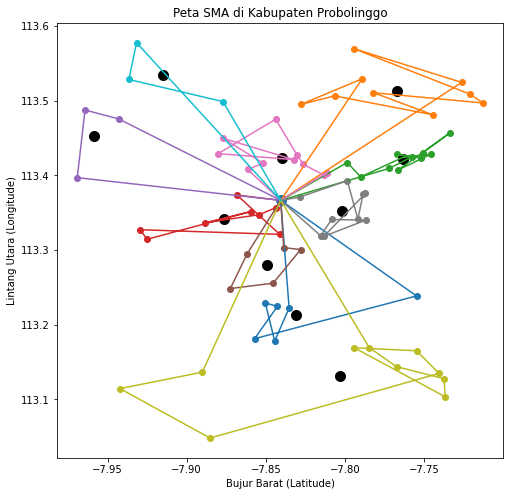
\includegraphics[width=0.5\textwidth]{Gambar/hasil_mtsp/10}
\caption{Perjalanan dibagi 10 klaster}
\label{fig:hasil_mtsp10}
\end{figure}

\section{Total Jarak Yang Dihasilkan}
Setelah semua proses di atas selesai, dapat dibandingkan total jarak seperti pada Tabel \ref{tab:totaljarak}, pembagian dataset  menjadi 7 klaster menempati posisi peringkat pertama yang mempunyai nilai total jarak paling rendah di antara pembagian klaster yang lain. Untuk urutan jalur yang dihasilkan dapat dilihat pada langkah pembagian 7 klaster di atas yang hanya dapat ditempuh dengan $4,353294633$ satuan. Daftar kode dari titik-titik SMA dapat dilihat pada Lampiran \ref{lampiran1}.

\begin{table}[H]
\centering
\footnotesize
\begin{tabular}{ccccc}
\rowcolor[HTML]{4472C4} 
\cellcolor[HTML]{4472C4}{\color[HTML]{FFFFFF} } &
  \cellcolor[HTML]{4472C4}{\color[HTML]{FFFFFF} } &
  \cellcolor[HTML]{4472C4}{\color[HTML]{FFFFFF} } &
  \multicolumn{2}{c}{\cellcolor[HTML]{4472C4}{\color[HTML]{FFFFFF} \textbf{Titik Kumpul}}} \\
\rowcolor[HTML]{4472C4} 
\multirow{-2}{*}{\cellcolor[HTML]{4472C4}{\color[HTML]{FFFFFF} \textbf{Banyak Klaster}}} &
  \multirow{-2}{*}{\cellcolor[HTML]{4472C4}{\color[HTML]{FFFFFF} \textbf{Total Jarak}}} &
  \multirow{-2}{*}{\cellcolor[HTML]{4472C4}{\color[HTML]{FFFFFF} \textbf{Peringkat}}} &
  \cellcolor[HTML]{4472C4}{\color[HTML]{FFFFFF} \textbf{Latitude (X)}} &
  \cellcolor[HTML]{4472C4}{\color[HTML]{FFFFFF} \textbf{Longitude (Y)}} \\
1  & 10,0503  & 10 & -7,8221841 & 113,3570412 \\
\rowcolor[HTML]{D9E1F2} 
2  & 6,858777 & 9  & -7,8241236 & 113,3236903 \\
3  & 5,599878 & 8  & -7,8219762 & 113,3512877 \\
\rowcolor[HTML]{D9E1F2} 
4  & 5,010994 & 7  & -7,8215022 & 113,3644199 \\
5  & 4,805015 & 6  & -7,828521  & 113,3744846 \\
\rowcolor[HTML]{D9E1F2} 
6  & 4,43132  & 3  & -7,8265701 & 113,3475373 \\
7  & 4,353295 & 1  & -7,8331118 & 113,3721289 \\
\rowcolor[HTML]{D9E1F2} 
8  & 4,398984 & 2  & -7,8358502 & 113,3704048 \\
9  & 4,48243  & 4  & -7,8321462 & 113,356253  \\
\rowcolor[HTML]{D9E1F2} 
10 & 4,780413 & 5  & -7,8406976 & 113,3665328
\end{tabular}
\caption{Total jarak dengan jumlah pembagian klaster yang berbeda}
\label{tab:totaljarak}
\end{table}

\section{Penyebab Rute Kurang Optimal}

Dalam penelitian ini dapat kita lihat bahwa hasil masih kurang optimal dalam penerapan algoritma genetika. Penyebabnya adalah terlalu banyak titik tujuan dalam sekali perjalanan, karena menurut penelitian sebelumnya penggunaan algoritma genetika keefektifannya akan semakin menurun jika digunakan dalam skala kota besar \cite{inproceedings}. Dalam penelitian ini hal tersebut dapat diminimalisir dengan meningkatkan banyak populasi pada tahap algoritma genetika. Namun hal tersebut juga masih memiliki keterbatasan yaitu waktu pemrosesan algoritmanya yang semakin lama.